\section{基于GRU的燃煤机组汽轮机系统状态监测方法}
\label{sec:gru_monitoring_v2}

\subsection{引言}

燃煤机组汽轮机系统承担着将高温高压蒸汽热能转换为机械能并驱动发电机发电的核心任务，其运行状态直接关系到机组的安全性、经济性及负荷调节能力。随着新能源高比例并网和电网调峰需求持续增加，燃煤机组由长期稳定负荷运行逐步转向频繁升降负荷、宽负荷区间运行。在此过程中，主蒸汽压力与温度、再热蒸汽状态、调节阀开度、机组负荷以及凝汽器冷端条件等边界均会发生持续变化，汽轮机各级汽缸压力、排汽温度、抽汽参数以及缸体温度等状态量也随之呈现明显的非线性和动态响应特征。已有研究表明，汽轮机在不同负荷和运行边界下具有显著不同的正常状态分布，因此仅依据固定阈值或单一设计工况进行状态判别，难以有效区分正常工况迁移与真实设备异常\cite{Cao2016LastStageNormalValue,Dettori2017MonitoringModels,Chen2023AdaptiveTransfer}。

从故障诊断链路看，状态监测建模的核心作用并非单纯提高某一参数的预测精度，而是建立给定运行边界条件下设备正常状态的动态参考。通过正常运行数据学习运行边界与设备状态之间的映射关系，可以获得设备在当前工况下应具有的正常状态输出；后续再将模型输出与实际运行数据进行比较，即可形成能够削弱工况变化影响的状态偏差信息。该思想与汽轮机正常值模型、在线性能监测及基于预测误差的异常检测研究具有一致性\cite{Jiang2014DataReconciliation,Ko2022DynamicThresholdAE,Zhai2024CAEWarning}。因此，在开展基于知识图谱和图卷积网络的故障分类前，有必要首先建立稳定、准确且具有良好工况适应性的汽轮机系统健康状态监测模型。

汽轮机系统由多个具有不同运行机理和边界条件的设备共同组成。若将全系统大量DCS测点无差别输入单一黑箱模型，虽然能够利用较多统计相关信息，但设备物理边界、参数归属以及上下游因果关系容易被弱化，不利于后续故障传播分析和模型解释。Zhang等在大型汽轮机全工况建模研究中同样依据系统组成和设备耦合关系，将汽轮机系统划分为汽轮机本体、回热设备、抽汽管路和凝汽器等多个子模型，并通过设备间参数传递形成系统整体模型\cite{Zhang2018AllCondition}。借鉴这一设备级组织思想，本文按照实际热力边界划分建模对象，将上游直接热力边界及本级操作量作为输入，将设备内部状态、出口状态及关键热力接口状态作为输出，形成面向燃煤机组汽轮机系统的统一状态监测建模框架。

考虑到汽轮机热力过程具有显著的时间相关性，本文采用门控循环单元（Gated Recurrent Unit, GRU）作为设备级状态监测的主要模型。GRU通过更新门和重置门实现对历史状态的选择性保留，在较紧凑的参数规模下能够提取连续运行数据中的动态信息\cite{Cho2014GRU}。同时，为评价不同类型网络在汽轮机状态监测任务中的适用性，选取ANN、TCN以及iTransformer-small作为对比模型。后文首先介绍汽轮机系统结构、主要设备及状态监测参数，随后给出设备级建模原则和GRU模型原理，最后以超高压缸（Very High Pressure Cylinder, VHP）作为代表性对象，详细展示输入输出定义、模型训练及状态监测效果。VHP在本章中承担的是系统级建模方法的典型算例角色，本文所提出的建模思想面向整个燃煤机组汽轮机热力系统。

\subsection{燃煤机组汽轮机系统及状态监测建模对象}
\label{subsec:turbine_system_and_objects}

\subsubsection{汽轮机本体及主通流过程}

本文研究对象为某大型二次再热燃煤机组汽轮机系统。汽轮机主通流由主蒸汽系统、超高压缸VHP、一次再热系统RH1、高压缸HP、二次再热系统RH2、中压缸IP、低压缸LP以及凝汽器共同组成。锅炉产生的高温高压主蒸汽经主汽门和调节阀进入VHP，在通流级组内膨胀做功后形成超高压缸排汽；排汽进入一次再热系统重新吸收热量，随后进入HP继续膨胀。HP排汽经二次再热后进入IP，并进一步流入LP做功，最终低压缸末级排汽进入凝汽器形成冷端边界。上述过程构成汽轮机最主要的蒸汽能量传递链路。

从状态监测角度看，主通流不同位置的压力、温度和流量参数具有明确的设备归属和物理含义。主蒸汽压力、主蒸汽温度和主蒸汽流量决定VHP入口的热力边界，调节阀开度反映本级配汽状态；VHP叶片级压力及排汽压力能够表征缸内膨胀和通流状态，排汽温度则综合反映入口热力条件、膨胀做功和通流效率等因素的影响。VHP排汽进一步构成一次再热系统的入口边界，因此冷再管段的压力和温度不仅是VHP出口状态，也是下游再热设备的重要接口状态。类似地，一次高温再热参数决定HP入口边界，二次再热参数决定IP入口边界，LP末级排汽状态与凝汽器背压共同构成低压缸及冷端系统之间的直接耦合关系。

因此，汽轮机本体状态并非由单一测点决定，而是由入口边界、阀门操作、级组压力分布、排汽状态以及相邻设备接口参数共同反映。不同状态变量所对应的物理过程具有明显差异：压力参数对流量与阀门动作响应较快，蒸汽温度同时受传热和膨胀过程影响，缸体金属温度则具有更强的热惯性和历史工况依赖。上述差异决定了汽轮机状态监测需要同时考虑多变量耦合与时间动态特征。

\subsubsection{抽汽回热、给水及冷端系统}

汽轮机系统除主通流外，还通过多级抽汽与回热系统、给水系统和凝汽器冷端系统形成复杂的能量耦合网络。汽轮机各级抽汽从不同压力级引出，分别进入高压加热器、低压加热器及除氧器，用于逐级提高凝结水和给水温度，减少锅炉侧加热所需热量。李萍关于大型凝汽式汽轮机系统建模的研究也指出，回热系统以各级抽汽为热源，给水加热器和除氧器共同构成连接汽轮机本体与锅炉给水系统的重要能量传递环节。对于状态监测而言，抽汽压力和温度既反映对应汽轮机级组的通流状态，也直接影响回热设备的换热性能和下游给水状态。

凝汽器是汽轮机低压排汽的终端设备，其主要作用是将低压缸排汽凝结为水并维持较低排汽压力。凝汽器真空或背压受循环水入口温度、循环水流量、换热面清洁程度、真空系统运行状态等因素影响，其变化会反向作用于低压缸末级膨胀过程。Zhang等构建汽轮机全工况系统模型时，将循环水温度、循环水流量、凝结水系统参数及凝汽器状态作为冷端子模型的重要边界，说明冷端条件与汽轮机本体运行状态之间存在不可忽略的耦合关系\cite{Zhang2018AllCondition}。

给水系统位于凝结水和锅炉之间，主要由凝结水泵、低压加热器、除氧器、给水泵及高压加热器等设备构成。给水泵对给水进行升压，高、低压加热器利用汽轮机抽汽对水进行逐级加热，形成“汽轮机抽汽—回热设备—给水参数—锅炉”的能量闭环。虽然本文第二章不逐一展开所有回热和给水设备的状态模型，但在系统级建模框架中仍保留这些设备及其热力接口，因为这些关系将在后续汽轮机知识图谱中用于描述设备归属、介质传递和故障传播路径。

综上，燃煤机组汽轮机系统不是相互独立设备的简单集合，而是由主通流、抽汽回热、给水和冷端系统共同组成的耦合热力网络。全工况汽轮机研究通常也需要根据实际系统组成将多个子设备模型通过边界参数连接起来\cite{Zhang2018AllCondition}。本文据此建立如图~\ref{fig:turbine_system_modeling_v2}所示的系统级研究对象，为设备划分、输入输出定义及后续知识图谱拓扑构建提供统一物理基础。

\begin{figure}[htbp]
    \centering
    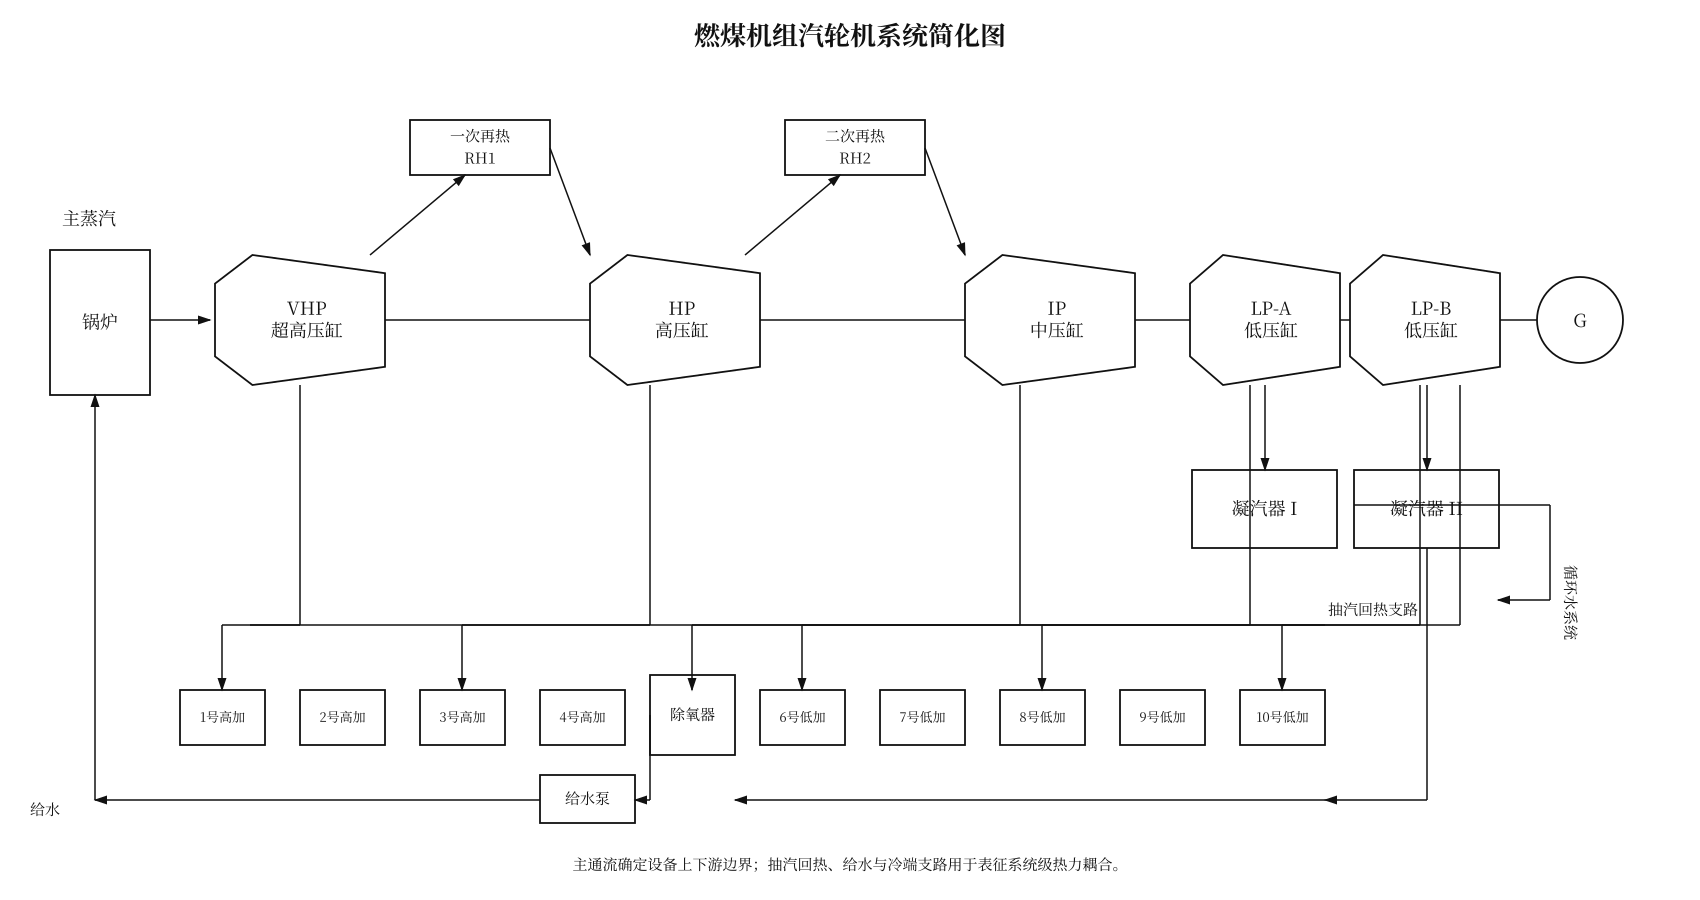
\includegraphics[width=0.98\textwidth]{figures/ch2/fig2_1_turbine_system_final.svg}
    \caption{燃煤机组汽轮机系统简化图}
    \label{fig:turbine_system_modeling_v2}
\end{figure}

\subsubsection{设备级状态监测建模思想}

针对上述多设备、多接口和多边界特性，本文采用设备级独立建模策略。该策略的核心思想是：以设备物理边界确定输入，以设备本体及出口状态确定输出，各设备分别利用真实DCS测量量建立状态映射模型，而不是将全部测点输入单一网络，也不采用“上一级模型预测值驱动下一级模型”的串联方式。这样既保留系统整体热力拓扑，又避免预测误差沿主通流逐级传播。

设汽轮机系统中第$d$个设备的直接热力边界向量为$\mathbf{B}^{(d)}_t$，本级操作量及总体运行条件向量为$\mathbf{U}^{(d)}_t$，则该设备在时刻$t$的输入表示为
\begin{equation}
    \mathbf{X}^{(d)}_t=\left[\mathbf{B}^{(d)}_t,\mathbf{U}^{(d)}_t\right].
    \label{eq:device_input_v2}
\end{equation}
设备内部状态、出口状态及关键热力接口状态记为$\mathbf{Y}^{(d)}_t$。对于动态模型，采用连续$L$个采样点构成输入序列
\begin{equation}
    \mathbf{X}^{(d)}_{t-L+1:t}
    =\left[
    \mathbf{X}^{(d)}_{t-L+1},\ldots,
    \mathbf{X}^{(d)}_{t}
    \right],
\end{equation}
模型映射可表示为
\begin{equation}
    \hat{\mathbf{Y}}^{(d)}_t
    =f_{\boldsymbol{\theta}_d}
    \left(\mathbf{X}^{(d)}_{t-L+1:t}\right),
    \label{eq:device_health_mapping_v2}
\end{equation}
式中，$f_{\boldsymbol{\theta}_d}(\cdot)$表示设备$d$对应的状态监测模型，$\boldsymbol{\theta}_d$为网络参数，$\hat{\mathbf{Y}}^{(d)}_t$为模型输出的设备状态估计值。

在测点选择过程中，本文遵循四项原则。第一，输入变量应具备明确的上游或本级因果边界含义，例如入口蒸汽压力、温度、流量及本级阀门开度；第二，不将本级近出口状态直接作为输入，以避免网络依赖强自相关变量获得表面上较高但缺乏诊断价值的预测精度；第三，设备输出不仅包含本体状态，还保留抽汽、再热和下游接口状态，使模型结果能够服务于系统级状态传播分析；第四，各设备均使用真实DCS测量量作为输入，不级联使用其他模型预测值，从而保证不同设备状态模型之间的误差相互独立。

按照该原则，可分别建立VHP、RH1、HP、RH2、IP、LP以及凝汽器等设备模型。各模型虽然输入输出维度不同，但均遵循“边界条件$B$+操作量$U$→设备状态$Y$”的统一建模范式。图~\ref{fig:device_model_framework_v2}给出了本文的设备级状态监测建模框架。

\begin{figure}[htbp]
    \centering
    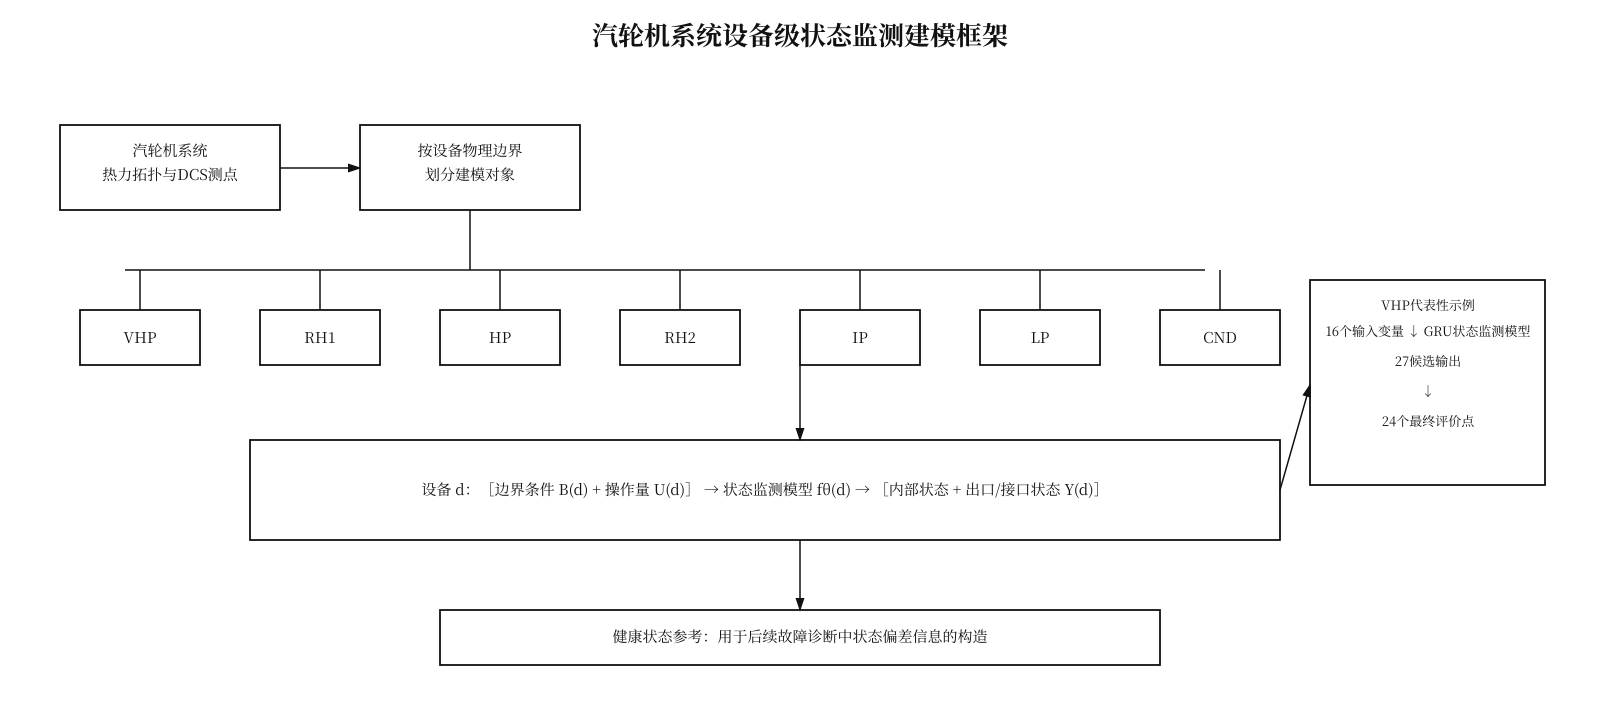
\includegraphics[width=0.92\textwidth]{figures/ch2/fig2_2_device_model_framework_final.svg}
    \caption{汽轮机系统设备级状态监测建模框架}
    \label{fig:device_model_framework_v2}
\end{figure}

\subsection{基于GRU的动态状态监测模型}
\label{subsec:gru_model_v2}

\subsubsection{循环神经网络的动态建模思想}

汽轮机DCS数据本质上属于多变量时间序列。对于压力、温度、阀位和流量等参数，当前状态不仅与当前时刻的运行边界相关，还会受到前一段时间内负荷变化和设备热惯性的影响。传统前馈神经网络将各时刻样本相互独立处理，难以显式保留跨时间步的信息。循环神经网络（Recurrent Neural Network, RNN）通过在隐藏层引入递归连接，使上一时间步的隐藏状态能够参与当前时间步计算，从而形成时间信息传递机制。

给定时间序列样本$\{\mathbf{x}_t,\mathbf{y}_t\}_{t=1}^{N}$，传统RNN的隐藏状态可表示为
\begin{equation}
    \mathbf{h}_t=\phi
    \left(\mathbf{W}_{xh}\mathbf{x}_t+
    \mathbf{W}_{hh}\mathbf{h}_{t-1}+\mathbf{b}_h\right),
\end{equation}
输出为
\begin{equation}
    \hat{\mathbf{y}}_t=
    \mathbf{W}_{hy}\mathbf{h}_t+\mathbf{b}_y,
\end{equation}
其中，$\mathbf{h}_t$为当前隐藏状态，$\mathbf{h}_{t-1}$为上一时间步隐藏状态，$\mathbf{W}_{xh}$、$\mathbf{W}_{hh}$和$\mathbf{W}_{hy}$分别表示输入到隐藏层、隐藏状态递归连接以及隐藏层到输出层的权重矩阵，$\phi(\cdot)$为非线性激活函数。吴婷婷在中速磨煤机动态建模研究中同样利用RNN隐藏状态的递归关系描述过程时间相关性，其基本思想是通过相邻时间步之间的信息传递提取动态过程特征。

传统RNN在较长时间序列训练时可能出现梯度衰减或梯度爆炸，使模型难以保留较长时间尺度的信息。GRU在RNN基础上引入门控机制，通过重置门和更新门对历史状态进行选择性处理，在结构上比LSTM更加紧凑，因此适用于本研究的小型设备级动态模型\cite{Cho2014GRU}。

\subsubsection{GRU门控机制}

设$t$时刻输入为$\mathbf{x}_t$，前一时间步隐藏状态为$\mathbf{h}_{t-1}$。GRU首先通过重置门$\mathbf{r}_t$控制历史信息在候选状态计算中的参与程度：
\begin{equation}
    \mathbf{r}_t=
    \sigma\left(
    \mathbf{W}_r\mathbf{x}_t+
    \mathbf{U}_r\mathbf{h}_{t-1}+
    \mathbf{b}_r
    \right),
    \label{eq:gru_reset_v2}
\end{equation}
其中，$\sigma(\cdot)$为Sigmoid函数。当$\mathbf{r}_t$中元素接近0时，对应历史状态在候选状态计算中的作用被削弱；当其接近1时，则更多保留前一时间步信息。

更新门$\mathbf{z}_t$用于控制上一隐藏状态与当前候选状态之间的信息融合比例：
\begin{equation}
    \mathbf{z}_t=
    \sigma\left(
    \mathbf{W}_z\mathbf{x}_t+
    \mathbf{U}_z\mathbf{h}_{t-1}+
    \mathbf{b}_z
    \right).
    \label{eq:gru_update_v2}
\end{equation}
在得到重置门后，候选隐藏状态$\tilde{\mathbf{h}}_t$计算为
\begin{equation}
    \tilde{\mathbf{h}}_t=
    \tanh\left[
    \mathbf{W}_h\mathbf{x}_t+
    \mathbf{U}_h\left(
    \mathbf{r}_t\odot\mathbf{h}_{t-1}
    \right)+\mathbf{b}_h
    \right],
    \label{eq:gru_candidate_v2}
\end{equation}
式中，$\odot$表示Hadamard乘积。当前隐藏状态最终由
\begin{equation}
    \mathbf{h}_t=
    (1-\mathbf{z}_t)\odot\mathbf{h}_{t-1}
    +\mathbf{z}_t\odot\tilde{\mathbf{h}}_t
    \label{eq:gru_hidden_v2}
\end{equation}
得到。由式~\eqref{eq:gru_hidden_v2}可见，更新门决定了历史状态与新候选状态在当前隐藏表示中的占比，使模型能够根据数据自动选择保留较长期趋势信息或快速响应新的运行边界变化。

对于汽轮机状态监测任务而言，主蒸汽压力、阀门开度和流量等变量可能在负荷调整时快速变化，而缸体温度、部分蒸汽温度具有明显的热惯性。GRU并不人为规定某一变量应采用多长的时间滞后，而是在训练过程中通过门控权重学习不同时间步信息对当前状态输出的综合贡献。因此，相比仅使用当前时刻输入的静态ANN，GRU更适合描述宽负荷运行中“快速边界变化—缓慢热状态响应”并存的动态关系。

\subsubsection{时序样本组织与多输出映射}

本文GRU模型的输入不是单一时刻向量，而是由连续24个采样点组成的多变量时间窗口。设每个时间步包含$m$个输入变量，则单个输入样本可写为
\begin{equation}
    \mathbf{X}_t=
    \left[
    \mathbf{x}_{t-23},
    \mathbf{x}_{t-22},\ldots,
    \mathbf{x}_t
    \right]^\mathrm{T}
    \in\mathbb{R}^{24\times m}.
\end{equation}
对于VHP算例，$m=16$。序列依次输入同一组参数共享的GRU单元，得到各时间步隐藏状态$\mathbf{h}_{t-23},\ldots,\mathbf{h}_{t}$。本文采用最后一个时间步的隐藏状态$\mathbf{h}_t$作为当前窗口的动态特征表示，并进一步经过LayerNorm、Dropout和线性映射得到多维状态输出：
\begin{equation}
    \hat{\mathbf{y}}_t=
    \mathbf{W}_o\,
    \mathrm{Dropout}
    \left[
    \mathrm{LayerNorm}(\mathbf{h}_t)
    \right]+\mathbf{b}_o.
    \label{eq:gru_output_v2}
\end{equation}
多输出结构使同一设备的多个状态变量能够共享GRU提取的动态特征，网络无需为每个压力或温度测点单独训练一套模型。一方面可减少模型数量；另一方面，多个状态输出通过共享隐藏表示进行联合学习，有利于利用设备内部不同测点之间的相关信息。

\subsubsection{数据标准化与损失函数}

汽轮机状态监测变量包含压力、温度、流量、阀门开度和功率等不同物理量，其量纲和数值范围差异较大。若直接使用原始数据训练网络，大尺度变量会在梯度更新中占据更大权重，不利于多输出模型同时学习不同状态。因此，本文分别对输入和输出变量进行标准化。对于任一变量$x$，标准化形式为
\begin{equation}
    x^{*}=\frac{x-\mu_x}{\sigma_x},
\end{equation}
其中，$\mu_x$和$\sigma_x$分别为训练数据中该变量的均值和标准差。所有标准化参数仅由训练数据确定，并在验证集和测试集上固定使用，以避免测试信息泄露。

GRU模型采用标准化空间中的均方误差（Mean Squared Error, MSE）作为回归损失。设批次中包含$N_b$个样本，每个样本包含$q$个输出变量，则回归损失定义为
\begin{equation}
    \mathcal{L}_{\mathrm{MSE}}=
    \frac{1}{N_b q}
    \sum_{i=1}^{N_b}
    \sum_{j=1}^{q}
    \left(
    y^{*}_{ij}-\hat{y}^{*}_{ij}
    \right)^2.
    \label{eq:mse_loss_v2}
\end{equation}
采用标准化输出计算MSE后，各输出维度在训练阶段处于近似统一尺度，从而避免压力与温度量纲差异直接主导网络权重更新。模型评价阶段再将预测结果反标准化至原始物理单位，并分别计算$R^2$、RMSE和MAE。

\subsubsection{模型训练与参数更新}

GRU属于时间展开的循环网络，模型训练通过时间反向传播（Back Propagation Through Time, BPTT）实现。对长度为24的输入序列完成前向计算后，损失函数首先由多输出预测结果得到，随后梯度从输出层反向传播至LayerNorm、GRU以及各时间步共享参数。由于同一GRU参数在24个时间步重复使用，各时间步对损失的贡献会在反向传播过程中累积，从而共同更新门控权重和隐藏状态映射参数。

本文采用AdamW优化器更新网络参数，初始学习率为$1\times10^{-3}$，权重衰减系数为$1\times10^{-4}$。模型选择阶段使用ReduceLROnPlateau策略，根据验证损失变化自适应降低学习率；同时采用梯度裁剪，将梯度范数限制在5.0以内，以降低循环网络训练过程中梯度爆炸风险。训练月按时间顺序划分模型拟合区间和验证区间，通过验证损失确定最佳训练轮次。获得最佳轮次后，再使用完整训练月数据按照相同轮次重新训练最终模型，并在独立测试月份上进行评价。

图~\ref{fig:gru_architecture_v2}给出了本文GRU状态监测模型结构。真实网络由单层GRU构成，输入张量维度为$24\times16$，隐藏状态维数为32，GRU输出经过LayerNorm和Dropout(0.05)后连接27维线性层，总可训练参数量为5755。需要特别说明的是，27维为实际网络训练的候选输出维度；最终24个状态点是在预测完成后根据诊断节点冻结规则剔除3个候选温度点形成，因此本文不将网络结构错误写为Linear(24)。

\begin{figure}[htbp]
    \centering
    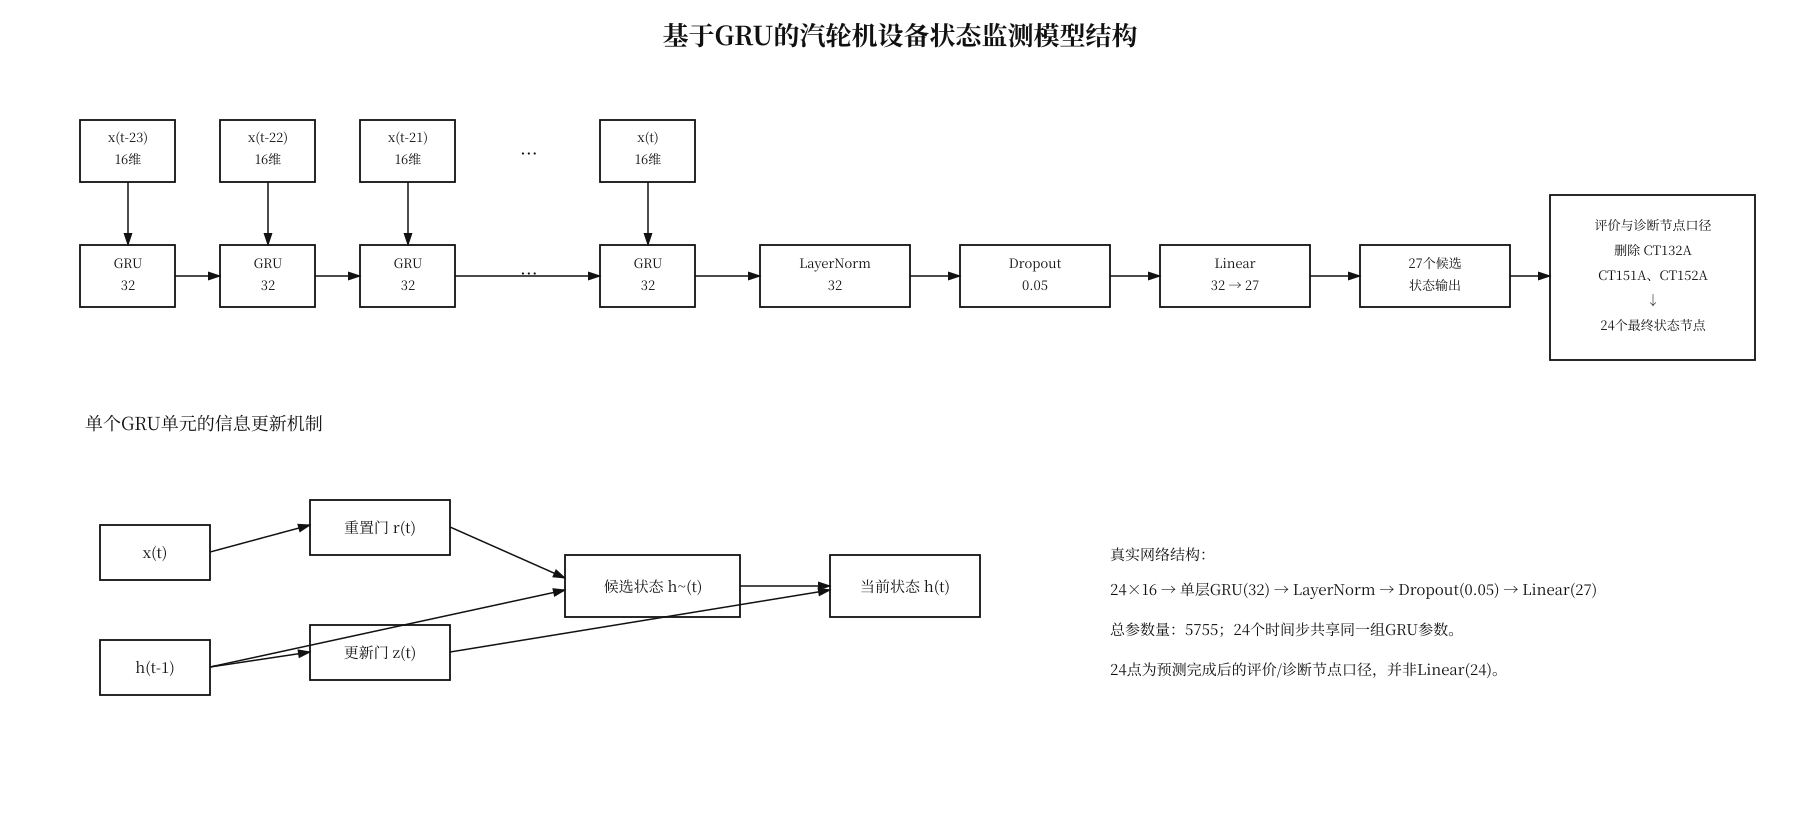
\includegraphics[width=0.98\textwidth]{figures/ch2/fig2_4_gru_architecture_final.svg}
    \caption{基于GRU的汽轮机设备状态监测模型结构}
    \label{fig:gru_architecture_v2}
\end{figure}

\subsubsection{对比模型}

为评价不同特征提取机制在VHP状态监测中的适用性，本文设置ANN、TCN和iTransformer-small三类对比模型。ANN采用两层全连接隐藏层，不显式利用历史时间信息，可作为静态映射基线；TCN通过因果卷积和膨胀卷积在固定时间窗口内提取局部与多尺度时序特征\cite{Bai2018TCN}；iTransformer-small将变量作为token，通过多头注意力学习变量间依赖关系，是轻量化注意力时序基线\cite{Liu2024iTransformer}。本文不在正文逐一展开三类对比模型的完整算法推导，而在实验设置中给出其主要网络参数，以保证第二章理论重心集中于GRU状态监测模型。

\subsection{以超高压缸为例的状态监测模型构建}
\label{subsec:vhp_case_v2}

\subsubsection{VHP运行过程与状态监测参数}

VHP位于汽轮机主通流起始端，其入口直接承接锅炉主蒸汽边界，出口与一次再热系统相连，同时通过一级抽汽支路与高压回热系统发生能量交换。因此，VHP既能够反映主蒸汽和调节阀作用下的汽轮机本体通流状态，又包含抽汽和再热两个典型热力接口，适合作为设备级状态监测方法的代表性对象。

在入口侧，A/B侧主蒸汽压力和温度表征进入VHP的热力状态，主蒸汽流量反映当前蒸汽通量，机组有功负荷用于描述整体运行水平，两侧调节阀实际位置则直接反映配汽机构操作状态。这些变量共同决定VHP在当前工况下的主要外部边界。与单独选取一个主蒸汽汇总值相比，保留A/B侧冗余压力和温度测点能够利用多测点信息降低单一仪表波动对模型输入的影响。

在输出侧，VHP本体测点首先包括叶片级压力、排汽蒸汽温度以及排汽管段压力和温度等参数，用于反映缸内膨胀及主排汽状态；一级抽汽支路参数包括抽汽压力、温度及逆止门前后管段温度，用于表征VHP向高压回热系统传递的抽汽状态；冷再接口参数位于VHP排汽至一次再热系统的连接位置，用于描述VHP向RH1传递的直接热力边界；此外，内外缸壁温及内部蒸汽温度等参数用于反映VHP金属部件和内部热状态，其变化相对压力参数具有更明显的热惯性。

这种测点组织方式与杨昊东在高压流化风机工程算例中的处理逻辑一致：并非仅罗列测点名称，而是根据设备过程将测点划分为边界、控制、负载、本体和接口等不同状态角色，并解释各类参数能够反映的物理过程。本文通过VHP主蒸汽边界、本体状态、一级抽汽接口、VHP--RH1接口及缸体热状态五个层面，构成较完整的VHP状态监测信息体系。

\subsubsection{VHP模型输入变量}

根据设备级建模原则和冻结后的变量定义，VHP状态监测模型最终采用16个输入变量。其中12个变量为A/B侧主蒸汽压力和温度冗余测点，包括A侧3个主蒸汽压力、B侧3个主蒸汽压力、A侧3个主蒸汽温度及B侧3个主蒸汽温度；操作变量包括两侧VHP调节阀实际位置；整体运行变量包括机组有功负荷及主蒸汽流量。

上述输入变量可以进一步划分为三类：第一类为直接热力边界，主要由主蒸汽压力、温度和流量构成，描述进入VHP的蒸汽状态；第二类为本级操作量，即VHP调节阀位置，描述配汽机构对通流的直接控制；第三类为总体工况量，即机组负荷，用于表征机组当前出力水平。当前主模型不引入高压旁路变量，也不将凝汽器背压作为VHP输入，其目的在于保持VHP模型输入与直接热力边界之间的一致性。

\begin{table}[htbp]
\centering
\caption{VHP状态监测模型输入变量构成}
\label{tab:vhp_inputs_v2}
\begin{tabular}{p{2.2cm}p{7.5cm}p{2.4cm}}
\toprule
类别 & 参数构成 & 数量\\
\midrule
主蒸汽压力 & A/B侧主蒸汽压力冗余测点 & 6\\
主蒸汽温度 & A/B侧主蒸汽温度冗余测点 & 6\\
操作量 & 两侧VHP调节阀实际位置 & 2\\
总体工况 & 机组有功负荷、主蒸汽流量 & 2\\
\midrule
合计 & --- & 16\\
\bottomrule
\end{tabular}
\end{table}

\subsubsection{VHP模型输出状态及分组}

VHP模型实际训练阶段设置27个候选状态输出，以尽可能覆盖设备本体、抽汽和再热接口的可观测状态。预测完成后，根据测点诊断相关性和最终节点冻结口径，删除CT132A、CT151A和CT152A三个候选温度点，最终保留24个状态参数用于本章性能统计及后续KG-GCN节点映射。

为了便于分析不同物理过程下模型性能，最终24个状态点划分为四组：Y1为VHP本体及主排汽状态，主要反映缸内膨胀和排汽过程；Y2为一级抽汽及1号高加接口状态，表征VHP向高压回热系统传递的热力信息；Y3为VHP至RH1冷再接口状态，表征主通流由VHP向一次再热系统传递的边界；Y4为VHP缸体与内部蒸汽状态，主要反映金属部件及内部蒸汽的热惯性过程。该分组既用于解释状态监测结果，也与后续知识图谱中“设备—参数—接口”的节点组织保持一致。

\subsubsection{数据集与预处理}

本文选取2024年5月正常运行数据建立VHP状态监测模型，并采用2024年6月作为独立测试时段。原始DCS采样周期为1~min，经运行状态筛选和数据质量处理后，训练月份包含43911条有效记录，测试月份包含42710条有效记录。训练月份负荷范围为280.986--1029.905~MW，测试月份负荷范围为285.910--1009.141~MW，能够覆盖较宽的正常运行区间。

时序模型以连续24个采样点构造一个序列样本。为保证序列的实际时间连续性，对存在时间戳间隔异常、缺失或重复的窗口予以剔除。完成窗口构造后，GRU训练集形成43759个序列样本，独立测试集形成42595个序列样本。输入和输出StandardScaler均仅根据训练数据拟合，并固定用于验证和测试数据。

本章目标是建立常规通流工况下的健康状态参考，因此当前主模型不将高压旁路运行模式纳入输入和训练对象。该处理使模型首先针对物理边界较清晰、数据规模较大的正常运行模式建立稳定基准，为后续故障诊断中的状态偏差分析提供一致的数据基础。

\subsubsection{模型参数与实验设置}

GRU模型采用时间窗口24、输入维度16、隐藏状态维数32、单层GRU、LayerNorm、Dropout(0.05)以及27维线性输出层，总参数量5755。训练采用AdamW优化器，初始学习率$1\times10^{-3}$，权重衰减$1\times10^{-4}$，批大小4096，梯度裁剪阈值5.0。模型选择阶段采用训练月前部数据进行参数拟合，后部数据作为验证集，并使用ReduceLROnPlateau动态调整学习率。验证损失最优的第161轮被确定为最终训练轮次，随后使用完整2024年5月数据重新训练模型。

对比模型主要参数见表~\ref{tab:model_settings_v2}。

\begin{table}[htbp]
\centering
\caption{不同状态监测模型的主要结构与参数}
\label{tab:model_settings_v2}
\small
\begin{tabular}{lp{10.5cm}}
\toprule
模型 & 主要结构及参数\\
\midrule
ANN & 两个全连接隐藏层32、16，LayerNorm，SiLU，Dropout=0.05；无显式历史时间窗口\\
GRU-RNN & 序列长度24，单层GRU，hidden size=32，LayerNorm，Dropout=0.05，Linear(27)\\
TCN & 序列长度24，3个因果深度可分离残差块，卷积核5，膨胀系数1/2/4\\
iTransformer-small & 序列长度24，1层Encoder，4头注意力，$d_{\mathrm{model}}=32$，前馈维数64\\
\bottomrule
\end{tabular}
\end{table}

模型采用决定系数$R^2$、均方根误差RMSE和平均绝对误差MAE进行逐测点评价：
\begin{equation}
R^2=1-\frac{\sum_{i=1}^{n}(y_i-\hat y_i)^2}{\sum_{i=1}^{n}(y_i-\bar y)^2},
\end{equation}
\begin{equation}
\mathrm{RMSE}=\sqrt{\frac{1}{n}\sum_{i=1}^{n}(y_i-\hat y_i)^2},
\end{equation}
\begin{equation}
\mathrm{MAE}=\frac{1}{n}\sum_{i=1}^{n}|y_i-\hat y_i|.
\end{equation}
由于24个输出同时包含MPa和$^{\circ}$C等不同物理量，RMSE与MAE仅用于单测点或相同物理量之间比较，不直接跨单位求宏平均；模型总体性能采用无量纲的24点宏平均$R^2$进行比较。

\subsection{算例分析与结果讨论}
\label{subsec:gru_results_v2}

\subsubsection{模型训练过程}

图~\ref{fig:gru_loss_v2}给出了模型选择阶段的训练损失和验证损失。模型训练初期损失快速下降，表明网络能够较快建立主蒸汽边界、阀门操作与VHP多状态输出之间的基本映射关系；随着训练轮次增加，训练损失和验证损失逐渐进入稳定区间，两者变化趋势总体一致。最低验证MSE为0.057533，对应epoch 161，此时训练MSE为0.043519。根据该最佳轮次，在完整训练月上重新训练后，第161轮完整训练集MSE为0.039283。

\begin{figure}[htbp]
    \centering
    % 建议最终换为figures/ch2/fig2_5_selection_loss.svg
    \caption{VHP的GRU状态监测模型训练与验证损失}
    \label{fig:gru_loss_v2}
\end{figure}

需要指出的是，训练损失仅反映模型对训练数据的拟合程度，不能单独证明健康状态模型具有足够泛化能力。因此本文进一步采用完整独立的2024年6月数据进行验证，并以多测点总体性能和典型热力状态作为主要评价依据。

\subsubsection{总体状态监测性能}

在最终24个状态点上，ANN、TCN、iTransformer-small和GRU-RNN的测试集宏平均$R^2$分别为0.9087、0.9397、0.9356和0.9511。GRU取得四种模型中的最高总体精度，相较ANN提高0.0424，相较TCN和iTransformer-small分别提高0.0114和0.0155。逐点统计进一步显示，GRU在24个最终状态参数中有17个测点取得最高$R^2$，说明其优势并非仅由少数高精度测点拉高平均值。

按物理状态分组后，GRU在Y1 VHP本体及主排汽状态、Y2一级抽汽接口、Y3 VHP至RH1接口上的平均$R^2$分别为0.9581、0.9634和0.9569，均保持较高精度；Y4缸体与内部蒸汽状态平均$R^2$为0.8893。该差异具有明确的工程含义：压力和主流蒸汽温度对主蒸汽边界和阀门调节响应较直接，而缸体金属温度具有更强蓄热和滞后特性，24点时间窗口及当前边界变量仍难完全覆盖其长期热状态演化。

\subsubsection{典型状态参数预测结果}

为了避免只利用单一宏平均指标评价模型，本文从不同物理状态中选择代表性测点进行分析。超高压缸叶片级压力\#1测试集$R^2$达到0.9979，RMSE为0.1417~MPa，MAE为0.1046~MPa，说明主蒸汽边界、流量和阀门操作能够较充分解释该压力状态变化。

对于热惯性更明显的排汽温度，模型差异更加突出。超高压排汽蒸汽温度\#1上，ANN、TCN、iTransformer-small和GRU的$R^2$分别为0.8092、0.8492、0.8488和0.8676；排汽蒸汽温度\#3上，四种模型对应$R^2$分别为0.8840、0.9153、0.9135和0.9387。时序模型整体优于静态ANN，说明利用历史运行信息有助于描述VHP排汽温度的动态变化，而GRU在该类关键热状态上表现最优。

一级抽汽接口同样体现了设备级模型对外部热力接口的描述能力。一级抽汽逆止门后水平管管顶温度的GRU测试$R^2$为0.9529，优于ANN、TCN和iTransformer-small。该结果说明VHP状态监测模型不仅能够预测本体内部状态，也能够建立VHP向高压回热系统传递的抽汽状态正常参考。

对于超高压内缸壁温90\%处\#1，GRU测试$R^2$为0.7346，iTransformer-small为0.7483，明显低于压力和蒸汽温度测点。本文保留该相对困难状态而不进行选择性删除，其结果表明金属温度受历史负荷轨迹和热蓄积影响更为显著，也是当前数据驱动健康模型后续需要重点改进的状态类型。

\subsubsection{模型比较与健康状态模型选择}

综合比较结果表明，ANN能够建立运行边界与状态输出之间的基本非线性映射，但由于不显式利用历史序列，对排汽温度和缸体热状态等具有明显动态特征的变量表现相对较弱；TCN利用因果卷积改善了时序特征提取能力，总体性能显著优于ANN；iTransformer-small在部分高精度压力测点上取得最优结果，体现了注意力机制对变量间关系建模的优势，但在当前小型网络和数据规模下整体宏平均性能略低于GRU。

GRU在保持5755个参数的小型网络规模下取得最高24点宏平均$R^2$，并在多数具有较明显热动态特征的状态点上表现稳定。结合后续故障诊断需求，健康状态模型不仅要求总体精度高，还需要对不同运行边界下的多类状态输出保持相对一致的跟踪能力。因此，本文最终选取GRU作为汽轮机设备级状态监测的基础模型，其预测输出将在后续KG-GCN章节中与实际运行数据进行比较，形成表征设备相对健康基准偏离程度的动态状态信息。

\subsection{本章小结}

本章面向燃煤机组汽轮机系统故障诊断对健康状态基准的需求，研究了基于GRU的设备级状态监测建模方法。首先从主通流、抽汽回热、给水和冷端系统出发，对汽轮机系统主要设备及参数之间的热力联系进行了分析，明确了不同设备的边界条件、操作变量、内部状态和关键热力接口。在此基础上，提出按照物理边界划分建模对象的统一方法，将设备直接热力边界和本级操作量作为输入，将设备内部及出口状态作为输出，为系统级状态监测和后续故障传播分析建立一致的数据组织框架。

随后，针对汽轮机状态参数具有明显时序相关性的特点，介绍了RNN动态建模思想和GRU门控机制，并从时序样本组织、多输出映射、数据标准化、损失函数及BPTT训练等方面构建了完整的GRU状态监测模型。本文真实网络采用$24\times16\rightarrow$单层GRU(32)$\rightarrow$LayerNorm$\rightarrow$Dropout(0.05)$\rightarrow$Linear(27)结构，总参数量5755。

最后以VHP为代表性对象开展工程验证。2024年5月训练、2024年6月独立测试结果表明，GRU在最终24个状态参数上的宏平均$R^2$达到0.9511，高于ANN、TCN及iTransformer-small，并在24个状态点中的17个点取得最高$R^2$。结果表明，GRU能够较好描述VHP本体、一级抽汽和冷再接口状态的正常动态响应，可作为后续汽轮机系统故障诊断的健康状态参考模型。